\documentclass[a4paper,12pt]{article}
\usepackage[utf8]{inputenc}
\usepackage{algorithmic}
\usepackage{algorithm}
\usepackage{pst-plot}
\usepackage{graphicx}
\usepackage{endnotes}
\usepackage{graphics}
\usepackage{graphicx}
\usepackage{floatflt}
\usepackage{wrapfig}
\usepackage{amsfonts}
\usepackage{amsmath}
\usepackage{dsfont}
\usepackage{verbatim}
\usepackage{hyperref}
\usepackage{multirow}
\usepackage{pdflscape}
\usepackage{multicol}
\usepackage[bottom]{footmisc}

\usepackage{hyperref}
\hypersetup{pdfborder={0 0 0 0}}

\pdfpagewidth 210mm
\pdfpageheight 297mm 
\setlength\topmargin{0mm}
\setlength\headheight{0mm}
\setlength\headsep{0mm}
\setlength\textheight{250mm}	
\setlength\textwidth{159.2mm}
\setlength\oddsidemargin{0mm}
\setlength\evensidemargin{0mm}
\setlength\parindent{0mm}
\setlength\parskip{3mm}

\graphicspath{{./images/}}



%
% Title
%
\begin{document}
\begin{center}
	{\Large
	University of Tartu\\
	Faculty of Mathematics and Computer Science\\
	Institute of Computer Science\\}
	\vspace{6cm}
	{\Large Kristjan Korjus, Ilya Kuzovkin, Ardi Tampuu, Taivo Pungas}\\
	\vspace{1.0cm}
	{\Huge Replicating the Paper ``Playing Atari with Deep Reinforcement Learning"\textsuperscript{\Large{\cite{mnih2013playing}}}}\\
	\vspace{0.5cm}
	{\Large Technical Report}\\
	\vspace{1.0cm}
	{\large MTAT.03.291 Introduction to Computational Neuroscience}
	
\end{center}
\vspace{9cm}
\begin{center}
	{\large Tartu 2014}
\end{center}
\thispagestyle{empty}
\pagebreak



%
% Table of contents
%
\thispagestyle{empty}
\tableofcontents
\pagebreak



%
% Introduction
%
\section*{Introduction}
\addcontentsline{toc}{section}{Introduction}
In recent years the popularity of the method called \emph{deep learning}\textsuperscript{\cite{hinton2007learning}} has increased noticeably in the machine learning community. Deep learning was successfully applied to speech recognition\textsuperscript{\cite{dahl2012context}} and many other tasks in machine learning\textsuperscript{\cite{deng2013new}}. In all these studies the performance of the resulting system was better than other machine learning methods were able to achieve so far.

The core of the deep learning method is an artificial neural network. One of the properties, which gives this family of learning algorithms a special place, is the ability to extract ``meaningful" (from a human perspective) \emph{concepts} from the data by combining the features based on the structure of the data. The extracted concepts sometimes have clear interpretation and that makes us feel as if the machine has indeed \emph{learned} something. Here we step into the realm of artificial intelligence, the possibility of which never stops to fascinate our minds.

A recent work, which brings together deep learning and artificial intelligence is a paper ``Playing Atari with Deep Reinforcement Learning"\textsuperscript{\cite{mnih2013playing}} published by DeepMind\footnote{\url{http://deepmind.com}} company. The paper describes a system that combines deep learning methods and \emph{reinforcement learning} in order to create a system that is able to learn how to play simple computer games. It is worth mentioning that the system has access only to the visual information (screen of the game) and the scores. Based on these two inputs the system learns to understand which moves are good and which are bad depending on the situation on the screen. Notice that a human player uses exactly same information to evaluate her performance and adapt her playing strategy. The reported result shows that the system was able to master several different games and play some of them better than a human player.

This result can be seen as a step towards truly intelligent machines and thus it fascinates us. The goal of this project is to create an open-source analogue of such a system using the description provided in the paper.



%
% Bird-eye view
%
\pagebreak
\section{Overview of the system}
Before we go into the details, let us describe the overall architecture of the system and show how the building blocks are put together. 

\subsection{The task}

The system receives a picture of a game screen (an example is shown in Figure \ref{fig:breakoutscreen}) and chooses an action to take. It then executes this action and is told whether the score increased, decreased or did not change. Based on this information and playing a large number of games, the system needs to learn to improve its performance in the game.

\begin{figure}[h]
\centering
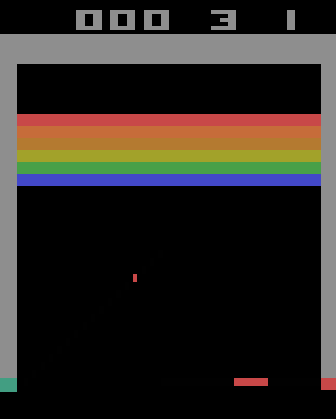
\includegraphics[width=3.5cm]{images/fig_gamescreen.png}
\caption{A game screen of Breakout.}
\label{fig:breakoutscreen}
\end{figure}

\subsection{Reinforcement learning}
\label{sec:reinforcementlearning}
In a reinforcement learning setting, an agent takes actions in an environment with the goal of maximising a cumulative reward. We tried to create a software agent that plays ATARI games in an emulator (the environment) and maximises its performance in the game, measured by its score in the games.

\subsubsection{Exploration-exploitation}
When the algorithm chooses between possible actions, it picks a ``learned" action with probability $1-\epsilon$ and a random action with probability $\epsilon$. The value of $\epsilon$ is gradually decreased as the algorithm learns to play better.

It is necessary to sometimes pick a random action to not get stuck in local reward maxima. At first, the value of $\epsilon$ is small and the agent takes random actions most of the time. This relatively high emphasis on exploration is necessary for the agent to collect information about the environment. When $\epsilon$ starts to decrease, the agent starts to apply its learned behaviour more and more, i.e. moving towards exploitation.

$\epsilon$ never reaches zero in the case of our agent, so it still does some exploration even when performing well in the game.

\subsection{Neural network}
The system uses a neural network to assign an expected reward value to each possible action. The input to the network at any time point consists of the last four preprocessed game screens the system received. This input is then passed through three successive hidden layers to the output layer. 

The output layer has one node for each possible action and the activation of those nodes indicates the expected reward from each of the possible actions - here, the action with the highest expected reward is selected for execution.

\subsection{Learning process}
\label{sec:learningprocess}
Under the fancy word ``neural network" hides a quite simple idea: a bunch of \emph{nodes} (neurons), each of them having some \emph{input} to perform a computation on and an \emph{output} where the result of the computation will be sent to, are connected to each other. Each connection has a \emph{weight}, which regulates how much one neuron can affect another. The very first layer of the network is usually called the \emph{input layer}. This is the place where we inject a data sample. Next to the input layer the network has several trickily connected \emph{hidden layers}. And the last layer is an \emph{output layer}, it gives us the final piece of information we wanted to know about the data sample we fed into the network. The resulting structure can be very complex, but the building blocks are always the same: neurons and connections between them.

We, as the builders of the system, usually know what we want it do: that is for each data sample we know what the final output should look like. Now the ``smart" neural network is the one able to produce the output we expect, the ``naive" network is the one which is not. The only thing that differs in those two are the \emph{weights} on the connections between the nodes. By changing them in accordance with our final goal the network goes from being ``naive" to being ``smart". This process in general in known as \emph{learning}.

To explain the concept of learning to the machine we introduce the notion of \emph{cost function} (or \emph{loss function}) which we will denote by $L$. Given the parameters of the network this function goes over the data samples, computes the outputs, compares these outputs with the expected ones and calculates how big is the error the system makes. The learning process can be represented as the process of \emph{minimizing} the cost function.

The obvious way to minimize a function is to try out all possible inputs to find the minimal output. Unfortunately the number of possible input is unfeasibly large. How to do it is a big question not only for our system. The whole brach on computer science called \emph{optimization} is dealing with this issue. One of the most popular technique used in this area is called \emph{gradient descent}.

The idea of gradient descent is rather trivial: at each \emph{iteration} of the learning algorithm it makes a small step in the ``direction" which makes the value of the loss function smaller. Thus by making enough steps the algorithm will reach an \emph{optimum}: a place from where a step in any direction will only increase the value of the loss function. Once this optimum is found we say that the learning has finished and the system is now as smart as it can be. It might happen that the optimum we found is not the best one (\emph{local optimum}), and there are bunch of techniques (for example \emph{Monte Carlo} methods) to find the \emph{global optimum}, but we will not dwell into this right now. 

Gradient descent uses the \emph{gradient} (multidimensional derivative) as it's core:
\begin{enumerate}
	\item Let the current configuration of the system be $\mathbf{w_0}$
	\item Compute the derivative (gradient) of the loss function at this point $L(\mathbf{w_0})$
	\item Look at the derivative with respect to each element $(w_1, \ldots, w_n) = \mathbf{w_0}$ and:
	\begin{enumerate}
		\item If the derivative is 0 then we should not touch this parameter of our system
		\item Otherwise move one step in the direction opposite to the derivative (positive slope -- decrease the parameter, negative slope -- increase the parameter)
	\end{enumerate}
	\item Repeat starting from the step 2. until the derivatives with respect to all parameters of the system are zeros (or close to zeros)
\end{enumerate}
Once this process is complete, we believe that our system has reached the optimal state: its parameters are configures in such way that it will give optimal performance on the dataset we have. In our system we will use variation of the idea of gradient descent called RMSProp, you will read about it later.



%
% Components
%
\pagebreak
\section{Components of the system}

In this section we intend to describe all the key components of the system in detail. This description should reflect all the choices we made, justify them and explain how the components work.



\subsection{Launching and communicating with ALE}
Just as we, humans, exchange information with a computer game by seeing the computer screen (input) and pressing the keys (output actions), the system needs to communicate with the Arcade Learning Environment that hosts the game.
\paragraph{}
Communication with ALE is achieved using two first-in-first-out (FIFO) pipes which must be created before ALE is launched. We create the pipes and launch ALE using the \verb=os= package of Python. The parameters given to ALE at execution must specify the way we want to communicate with ALE (FIFO pipes) and the location of the binary file containing the game to run (Breakout). In addition, we specify that we want ALE to return unencoded images, that only every 4th frame should be sent to us and whether the game window should be made visible.


\paragraph{}
The actual communication starts with a handshake phase, where we define the desired inputs (screen image and episode information) and ALE responds by informing us about the dimensions of the image. Thereafter the conversation between ALE and our agent consists in reading and deciphering inputs from \texttt{FIFO\_in} pipe and sending the chosen actions back through \texttt{FIFO\_out} pipe. The information is read from pipes as one long String, so deciphering is needed (cutting the input and converting the pieces into appropriate types). Similarly, the chosen action has to be transformed to an output string of specific format. If a game is lost, a specific ``reset" signal is sent to start the next game. When the desired number of games has been played, the communication with ALE can be terminated by closing the communication pipes. 



\subsection{Convolutional neural network}
Our system receives $4 \times 84 \times 84$ pixel values as input. In order to find relevant information from these four $84 \times 84$ images, we use convolutional neural networks (CNN)\textsuperscript{\cite{lecun1995convolutional}}. CNNs are a specific type of neural network that are particularly adapted to extracting features from images.

Unlike restricted Boltzmann machines (RBMs) that see their input as an 1D vector, a CNN treats the input images as 2D objects. These 2D matrices of pixel values are convolved with linear filters to obtain the activities of the next layer. For example, our first hidden layer is generated by convolving our images with sixteen different $8 \times 8$ filters, using a step of 4 pixels. This means that for each of the 16 different filters, we first take the top left $8 \times 8$ values of an image and linearly combine them with the filter, obtaining as a result one activity value. We then move 4 pixels to the right and multiply another $8  \times 8$ area from the image with the same filter.   When reaching the right edge of the image, we start again from the left, only 4 pixels lower. There are $8  \cdot 8 \cdot 4$ weights in a filter of this kind and the same weights (the same filter) is applied at different positions of the image, as described.

Each linear combination yields one activity value, so convolving an $84  \times 84$ image with an $8 \times 8$ filter with step 4 produces $20 \times 20$ topologically arranged values. As we apply 16 different filters, we end up with $16 \cdot 20 \cdot 20$ nodes in the first hidden layer of our convolutional network. 

An attentive reader will notice that our input consists of 4 images, not one. This means that each of our filters contains four weight matrices of size $8 \times 8$. The images will be convolved with the corresponding $8 \times 8$ matrix and the calculated activities are summed, so we end up with $16 \cdot 20 \cdot 20$ values as before.
%All in all, $W^{KL}_{ij}$ denotes the weight value connecting the pixel value on coordinates $(i,j)$ of the selected 8x8 area of the $L$-th image with the $K$-th feature map.

Last but not least, a linear rectifier is applied to the activity values, setting all negative values to 0.

The obtained sixteen $20 \times 20$ feature maps are thereafter convolved with 32 $4 \times 4$ filters. Using a step of 2, this yields $32 \times 9 \times 9$ activity values in the second hidden layer. As before, the filters are not 2-dimensional, instead they have $16 \times 4 \times 4$ values.

With these two convolutional layers we have reduced the number of nodes from $4 \times 84 \times 84$ to $32 \times 9 \times 9$. Functionally, after training the system we expect the nodes of the second hidden layer to represent spatiotemporal patterns relevant for successfully playing the game.

\begin{figure}[H]
	\centering
	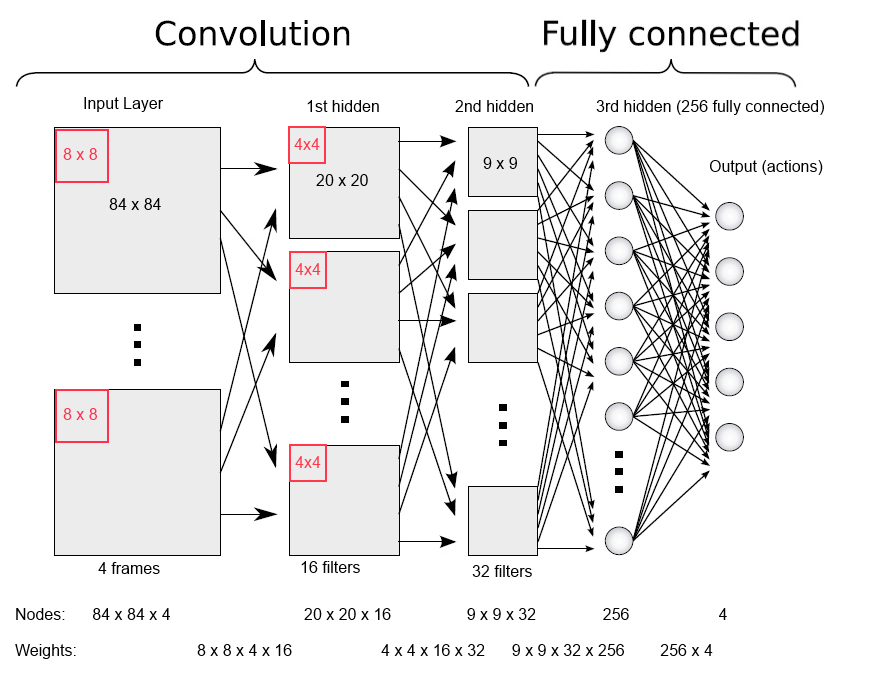
\includegraphics[width=\textwidth]{images/Convolutional_NN2.png}
	\caption{A diagram representing the organisation of the deep neural network used. The two last rows show the number of nodes and the number of independent weights.}
	\label{fig:neuralnet}
\end{figure}

\subsection{Q-learning}
In Section \ref{sec:reinforcementlearning} we introduced the notion of reinforcement learning: each time an agent performs an action, it receives a reward or punishment and updates its behavior rules accordingly. One very popular method for implementing this concept is called Q-learning\textsuperscript{\cite{watkins1992q}}.

The program is in a state $s_t \in \mathcal{S}$ and wants to know which action $a_t \in \mathcal{A}$ it should do to maximize the reward $r \in \mathds{R}$. So the typing of the function $Q$ is as follows:
$$Q: \mathcal{S} \times \mathcal{A} \rightarrow  \mathds{R}$$
and the actual implementation of this function is
$$Q_{t+1}(s_t, a_t) = Q_t(s_t, a_t) + \alpha\cdot(r_{t+1} + \gamma\cdot\max_{a}Q(s_{t+1}, a) - Q_t(s_t, a_t))$$
where
\begin{itemize}
	\itemsep 0em
	\item[] $Q_t(s_t, a_t)$ is the reward I thought I will get if I do action $a_t$ while being in state $s_t$. In our implementation, this is calculated using the deep neural network.
	\item[] $r_t+1$ is the reward I actually got for doing action $a_t$ while being in state $s_t$
	\item[] $\alpha$ is the learning rate
	\item[] $\gamma$ is a \emph{discount factor} which says how much should I take into consideration the future rewards along this path
	\item[] $max_{a}Q(s_{t+1}, a)$ is what I think will be the best reward available from the next state (future reward)
\end{itemize}

\subsection{Root Mean Squares of gradients (RMSProp)}
In Section \ref{sec:learningprocess} we have seen the logic of gradient descent update procedure. There are, however, problems with this approach. One of them is that once you have established and update vector $\mathbf{u}$ you might notice that for some components $u_i = \frac{\partial L(\mathbf{w})}{\partial w_i}$ it proposes huge changes and tiny changes for the others. It might be not very reasonable to use the same learning $\mu$ rate for all components. The idea of RMSProp is to come up with a separate learning rate $\mu_i$ for each of the components $u_i$.

If you can use all of your data to estimate the direction of the gradient, then you can cope with this problem by just using sign of the gradient $sign(\frac{\partial L(\mathbf{w})}{\partial w_i})$. This will ensure that all components of the gradient are treated equally. This approach is called \emph{rprop}. However we do not have the luxury of using all the data points in our loss function $L$: it would take too much time. This is where the idea of \emph{stochastic gradient descent} comes into play.


\subsubsection{Stochastic gradient descent}
As you know, if you have a set of differentiable functions, then the sum of these functions is also differentiable and the derivative of this function is equal to the sum of the derivatives of these functions:
$$\nabla f(\mathbf{w}, \mathbf{x}) = \displaystyle\sum\nabla g(\mathbf{w}, \mathbf{x_k})$$
where $\mathbf{x}$ is a set of data samples and $\mathbf{x_k}$ is one data sample. This fact allows us to take a sample from the dataset, compute updates $\mathbf{u}$ on it and then repeat this several time. At the end of the day it will produce the same results as if we had performed the gradient descent on the whole dataset at once.

Unfortunately rprop does not work with small sets of subsamples\textsuperscript{\cite{tieleman2012lecture}} (\emph{minibatches}). Although the blunt simplification of taking the gradient sign instead of the value works when we use the whole dataset (because it effectively converges to the average value of the magnitude of the update) it does not work on small random subsamples: there we could easily obtain an update which is too large compared to what we would like to have. The next build-up on top of the rprop idea is called \emph{rmsprop} and deals with that issue.

\subsubsection{RMSProp}
When we average the results obtained using rprop method we divide by the magnitude of the gradient. RMSProp proposes to keep track of previous gradients and divide updates not by the current magnitude, but the average magnitude over the last several updates (minibatches). This will allow to modify each component $u_i$ according to its previous magnitudes, preventing from taking it into account with too large or too small weight.


%
% Implementation
%
\pagebreak
\section{Implementation details}
The prototype of the system is built using \texttt{Python 2.7} with heavy usage of \texttt{theano}\textsuperscript{\cite{bergstra2010theano}} and \texttt{numpy}\textsuperscript{\cite{oliphant2007python}} libraries. Once the proof-of-concept stage is complete we will consider using \texttt{C++} if it will yield better performance. On Figure \ref{fig:classdiagram} we present current overall structure of the application. The subsections below will explain the particularities.

\begin{figure}[h]
	\centering
	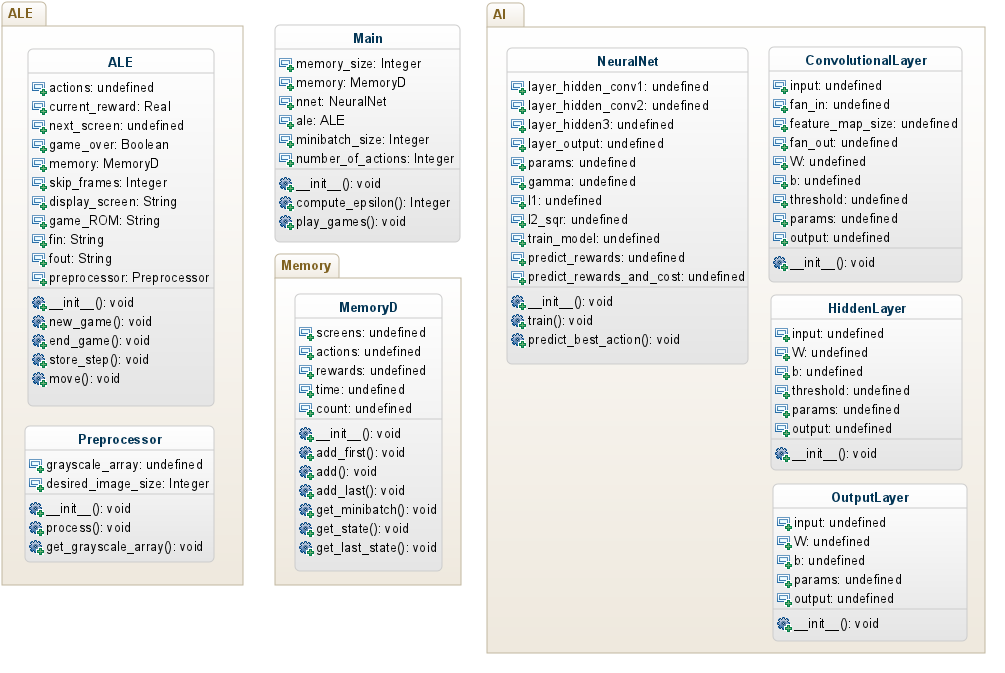
\includegraphics[width=\textwidth]{images/DeepMind-diag.png}
	\caption{Class diagram representing the overall structure of the application.}
	\label{fig:classdiagram}
\end{figure}


\subsection{Atari Learning Environment}
To simulate the game we use Atari Learning Environment (ALE)\textsuperscript{\cite{bellemare13arcade}}. It is a game simulator which allows to programmatically send player commands and receive the game output (image of the game screen, score, state of the game). Class \texttt{ALE} facilitates communication with the game emulator.


\subsection{Preprocessing}
\label{subsection_preproc}
The game screens are preprocessed by cropping the original $160 \times 210$-pixel image to a $160 \times 160$ region of interest, which is then downscaled to a $84 \times 84$ image.

The colors from ATARI's NTSC palette are converted to RGB using a conversion table
\footnote{\url{http://www.biglist.com/lists/stella/archives/200109/msg00285.html}}. The RGB representation is then converted to grayscale according to the weighted combination $0.21R + 0.71G + 0.07B$. This should produce a representation close to human perception (humans are more sensitive to green than other colours)\footnote{\url{http://www.johndcook.com/blog/2009/08/24/algorithms-convert-color-grayscale/
}}. An example of a preprocessed image is shown in Figure \ref{fig:breakoutpreprocessed}.

\begin{figure}[h]
\centering
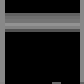
\includegraphics[width=2.5cm]{images/fig_preprocessedscreen.png}
\caption{A preprocessed game screen of Breakout.}
\label{fig:breakoutpreprocessed}
\end{figure}


\subsection{Memory}
On of the central parts of the applications if the memory, where game states, player actions and received rewards are stored. Class \texttt{MemoryD} is a structure where all this information is stored and implements methods for storing and extracting information.


\subsection{Neural network}
In our implementation of the neural network we heavily rely on the \texttt{Theano} toolbox. Theano allows to define, optimize, and evaluate mathematical expressions involving multi-dimensional arrays efficiently\footnote{\url{http://deeplearning.net/software/theano}}. We closely follow the deep learning tutorial\footnote{\url{http://www.deeplearning.net/tutorial}} to define and build the neural network. Classes \texttt{ConvolutionalLayer}, \texttt{HiddenLayer} and \texttt{OutputLayer} describe building block of the network and the \texttt{NeuralNet} class puts them together and provides function for training and using the neural network.

\subsection{Computing on GPU}
As you can imagine, the computations on a neural network are highly parallelizable due to the fact that you can compute each neuron independently. Also the learning process can be parallelized to evaluate several inputs at the same time to obtain several updates in one unit of time. Theano library is able to perform the highly parallel GPU computations.

\subsection{Running instructions}
For more technical details and running instruction please refer to our wiki \url{https://github.com/kristjankorjus/Replicating-DeepMind/wiki}


%
% Results
%
\pagebreak
\section{Results}
At this point of time we can not drive any conclusions about how well the system perform or is it functional at all. Before we will be able to estimate that we need to finish the system build-up and confirm that all the learning procedures work.

\subsection{Performance measures}
One possible measure will be to plot the score change over the time. If we will observe that over the time the system is able to score more during fixed-length time window than before, we will have a strong indication that the system is doing something reasonable.

\subsection{Comparison to human player}
Yet to be performed.

\subsection{Comparison to the original paper}
Yet to be performed.

\subsection{Applications and future usage}
We believe that the technique used in this system allows to solve wide variety of machine learning tasks. It will be interesting to test the system on machine learning benchmark datasets.



%
% Bibliography
%
\pagebreak
\addcontentsline{toc}{section}{Bibliography}
\bibliographystyle{alpha}
\bibliography{report}

\end{document}